% Generated mechanically from the reviewed Markdown source.
% Controller edits should be made in both source and LaTeX when material.

\section{MuralPresenter}

Figure~\ref{fig:release-workflow} gives the system overview. MuralPresenter first externalizes the task and deck state, then assigns only independently acceptable work to fresh Agent contexts, binds dependent pages to shared Group Agents, and closes residual relations through render-grounded review. Sections 3.1--3.3 respectively formalize the task and state projection, specify role boundaries, and define grouping, visual critique, and scope-based revision.

\subsection{The Long-Horizon Presentation Task}

We formulate presentation authoring as an interactive agentic task. Given a user request \(q\), optional attachments \(\mathcal{M}\), a language \(\ell\), and a target length \(N\), the system operates with tool library \(\mathcal{T}\) and persistent state \(\mathcal{S}\), producing a deck \(D=(s_1,\ldots,s_N)\) together with per-slide notes and renders.

The generation process is a multi-step trajectory \(\tau\) decomposed into four phases: \[
\tau \;=\; \tau^{\mathrm{ground}} \circ \tau^{\mathrm{plan}} \circ \tau^{\mathrm{gen}} \circ \tau^{\mathrm{review}},
\] corresponding to content grounding, deck-wide planning, grouped generation, and whole-deck review. A downstream phase does not begin until its dependencies are ready in \(\mathcal{S}\); the generation phase further decomposes into disjoint page-group trajectories \(\tau^{\mathrm{gen}}=\{\tau^{G_1},\ldots,\tau^{G_m}\}\) running in parallel, where \(\{G_1,\ldots,G_m\}\) partitions \(\{1,\ldots,N\}\) (§3.3).

State externalization grounds this phase ordering. Each accepted artifact \(d\) enters \(\mathcal{S}\) with a fixed producing phase and owner role. A role \(r\) reads only its declared projection: \[
\pi_r(\mathcal{S}) \;\triangleq\; \{d \in \mathcal{S} \mid d \text{ is in } r\text{'s declared read-set}\},
\] and model-generated writes target only its declared write-set. In implementation, \(\mathcal{S}\) corresponds to the deck's persistent state directory, each Skill's role card declares \(\pi_r\), and the delegation topology enforces which artifacts a fresh context receives; deterministic scripts may still derive or update shared state on behalf of any role. The projection thus formalizes the delegation contract—what each role is responsible for reading and producing—rather than hard filesystem isolation.

The task is \emph{long-horizon}: an opening thesis must resolve at the end, and terms or visual encodings defined early must be reused throughout. We write such a relation as a cross-slide dependency \(g_k=(a_k,T_k,\Phi_k)\): source page \(a_k\) establishes a decision, target set \(T_k\) consumes it, and predicate \(\Phi_k\) tests whether the relation holds. Deck-level consistency is then characterized by whether these dependencies close (§5); MuralPresenter's design turns on which roles bear joint responsibility for cross-slide dependencies at which lifecycle boundary.

\subsection{Skill-Driven Multi-Agent Collaboration}

MuralPresenter expresses responsibilities as pluggable Skills that specify when a role is triggered, which projection of \(\mathcal{S}\) it reads, what it produces, and the handback criterion. A separate Agent is opened only when work can be delivered and accepted independently; otherwise the Orchestrator proceeds with tools.

\textbf{Orchestrator.} Interprets user intent, coordinates grounding, plans the deck, delegates production, and accepts results—but does not search images, write pages, or judge pixels. Deterministic operations (parsing, downloading, rendering, building) are invoked directly as tools. Per-slide spoken scripts are fixed during planning and deterministically compiled into a unified speech artifact before production. Group Agents implement only the frozen visible-content contract without rewriting scripts. After render-grounded whole-deck Review, a final deterministic pass re-synchronizes the speech artifact.

\textbf{Material \& Research.} Material parses attachments into structured summaries; Research verifies only external facts that would change a conclusion. Both consolidate outputs into citable grounded knowledge. Neither role appears when no attachment and no external fact is at stake.

\textbf{Image.} Opened only when a page plan genuinely needs photographs or generated pictures; it isolates retrieval, generation, candidate comparison, and pixel inspection from the global trajectory.

\textbf{Group Agent.} Each Group Agent owns one page group and, along a single bounded trajectory \(\tau^{G_j}\), jointly generates and inspects all pages in that group (§3.3), maintaining within-group relations without negotiating with other groups. Independent groups run in parallel.

\textbf{Review.} After generation converges, a Review role that took no part in generation performs an independent whole-deck inspection in an isolated context, avoiding self-assessment bias (§3.3). The build tool then packages the final artifact and validates consistency. Figure~\ref{fig:release-workflow} connects these ownership boundaries to the complete authoring, revision, and delivery lifecycle.

\begin{figure*}[t]
\centering
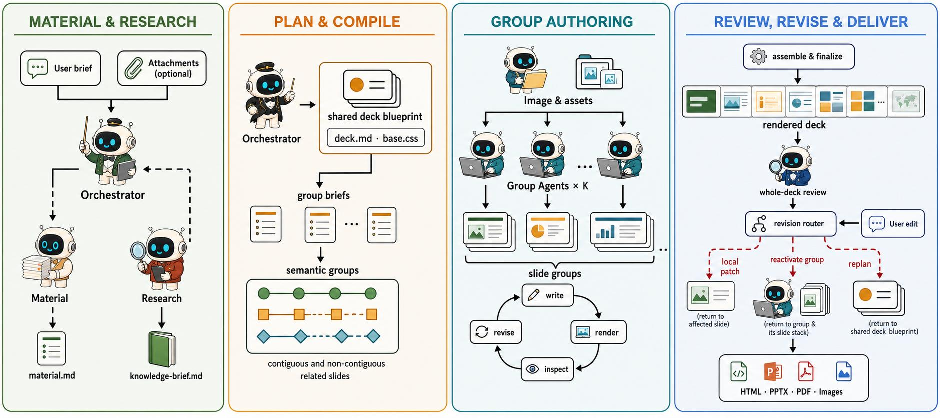
\includegraphics[width=0.90\textwidth]{figures/fig2_release_workflow.pdf}
\caption{\textbf{The full authoring and revision lifecycle in \sys{}.}
Material and Research ground inputs on demand; the Orchestrator writes the blueprint and group briefs; Image
prepares required bitmaps. Group Agents run parallel render--inspect--revise loops, whole-deck Review checks
cross-group relations, and the revision router replays the smallest responsible unit. Deterministic tools
transfer assets, render, validate, and package HTML, PPTX, PDF, and image delivery.}
\label{fig:release-workflow}
\end{figure*}


\subsection{Grouping, Visual Critique, and the Revision Loop}

\textbf{Dependency-aligned grouping.} MuralPresenter partitions the page set into complete, non-overlapping groups according to narrative, design, and asset affinity. Deck-level dependency closure decomposes into: \[
\mathrm{DC}(D)=\underbrace{\frac{1}{K}\!\!\sum_{k:\,\exists j,\,\{a_k\}\cup T_k\subseteq G_j}\!\!\mathbf{1}[\Phi_k\ \text{closed}]}_{\text{within-group: closed by one Group Agent}}
\;+\;
\underbrace{\frac{1}{K}\!\!\sum_{k:\,\nexists j,\,\{a_k\}\cup T_k\subseteq G_j}\!\!\mathbf{1}[\Phi_k\ \text{closed}]}_{\text{cross-group: backstopped by review}}.
\] The grouping goal is to pull as many strong dependencies as possible into the within-group term, leaving only a small number of cross-group relations to whole-deck review; we measure this gap in experiments (§6). Independent groups generate in parallel.

\textbf{Two-level visual critique.} Many defects surface only when rendered. MuralPresenter makes pixel inspection a first-class operation at two levels. Within a group, the Group Agent renders each page, revises until it holds in pixels, then reviews a group contact sheet for rhythm and repetition. At the deck level, Review inspects the full rendered deck in an isolated context; this independent-critic design also carries over to data synthesis (§4). Review is deliberately restrained: deterministic rendering imposes a hard gate only for CJK-font breakage; all other signals are returned as advice.

\textbf{Scope-based revision.} Post-generation edits reuse persistent state. Given an edit, the router conservatively infers an impact set \(I\): the directly touched pages plus any pages implicated through known cross-slide relations. Let the declared responsibility units be \(\mathcal{U} = \bigl\{\{i\} \mid i \in [N]\bigr\} \cup \{G_1,\ldots,G_m\} \cup \{[N]\}\), ordered by inclusion; the routing policy selects: \[
\mathrm{scope}(I) \;=\; \min_{U \in \mathcal{U}}\; U \quad \text{s.t.} \quad I \subseteq U.
\] This formalizes the implemented routing policy, not a learned optimizer: the system does not guarantee globally minimal cost or complete dependency knowledge, and escalates when impact is ambiguous. Concretely: a single-page patch goes through the Orchestrator; within-group relation changes reactivate the corresponding Group Agent \(\tau^{G_j}\); new facts or assets restart Research or Image on demand; structural changes (pages added, removed, reordered, or title chain altered) update the partition and trigger whole-deck review. Edit quality and preservation of untouched pages are tested in multi-turn experiments (§6). The final artifact is structured HTML, exportable to images, PDF, and PPTX.

\section{Long-Horizon Agentic Data Synthesis}

This section describes our data pipeline: task-dataset construction, trajectory synthesis with external verification, and multi-stage filtering (Figure~\ref{fig:data-synthesis}). We distinguish the controlled 9B corpus from the larger heterogeneous 27B training cohort.

\begin{figure}[H]
\centering
\begin{tikzpicture}
\node[inner sep=0] (datafig) {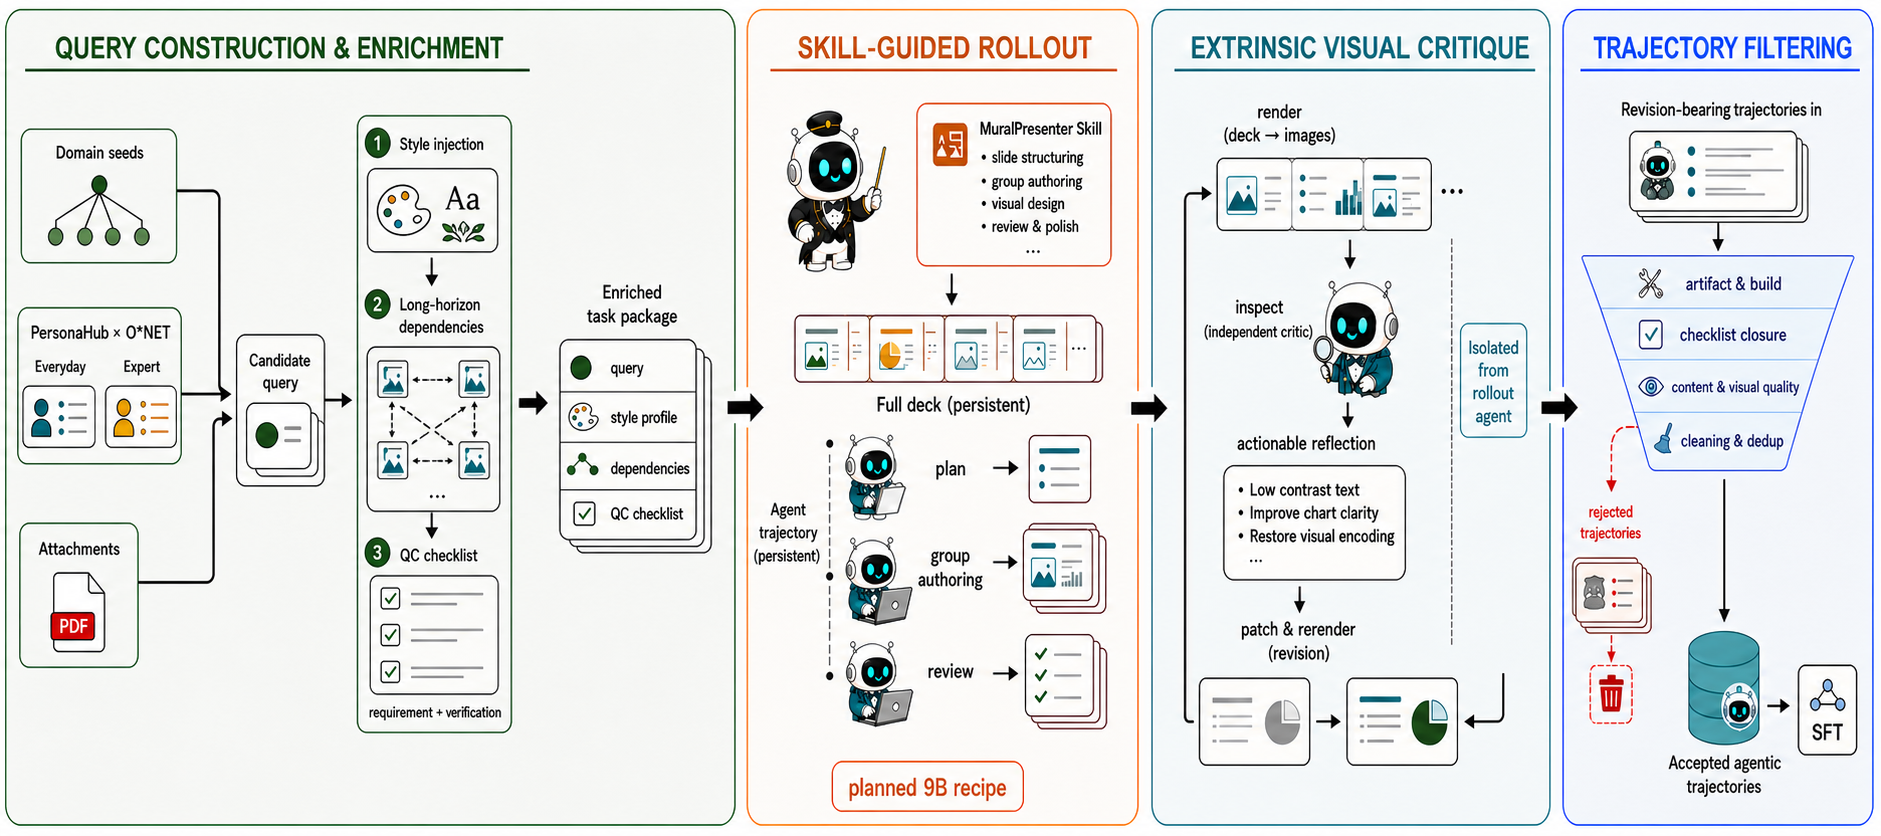
\includegraphics[width=\linewidth]{figures/fig3_long_horizon_agentic_data_synthesis.png}};
\node[fill=white,draw=auditorange,rounded corners=1.5pt,inner xsep=4pt,inner ysep=2pt,font=\scriptsize\sffamily,text=auditorange] at ($(datafig.south west)!0.493!(datafig.south east)+(0,0.43cm)$) {MuralPresenter-9B corpus};
\end{tikzpicture}
\caption{\textbf{Long-horizon agentic data synthesis.} Three query tracks feed a shared enrichment layer that injects a Style profile, constructs task-conditioned long-horizon dependencies, and compiles them into a checklist for downstream QC. A Skill-guided rollout preserves planning, group authoring, and review; an isolated visual critic induces render-grounded revisions; layered filtering retains only structurally complete trajectories that close the checklist. This controlled pipeline produces the MuralPresenter-9B corpus; the 27B cohort differs in teacher provenance and scale.}
\label{fig:data-synthesis}
\end{figure}

\subsection{Query Construction}

High-quality long-horizon training requires tasks whose structure is checkable across the deck. For MuralPresenter-9B, we construct candidate queries from three complementary tracks and then apply a shared enrichment layer. A Style profile sampled from a unified taxonomy is woven into the query as concrete guidance for color, typography, decorative motifs, and whitespace. The pipeline then constructs task-conditioned long-horizon dependencies, such as section quotas, narrative carry-over, cross-slide numeric consistency, motif continuity, loop closure, and explicit cross-slide references. We do not define long-horizon structure by a fixed number of constraints: each dependency records its type, concrete requirement, and closure condition. It is then compiled into a \texttt{longhorizon\_checklist} item specifying both the requirement and how downstream QC should verify it.

\textbf{Track 1: Domain-seed expansion.} From a hierarchical domain pool, seed topics expand into tasks spanning diverse disciplines and scenarios, emphasizing breadth and diversity.

\textbf{Track 2: Persona-driven real scenarios (PersonaHub \(\times\) O*NET).} Speaker personas are matched to tasks via the O*NET taxonomy in two tiers: a general everyday tier and an expert/elite tier with greater domain depth and longer dependency spans. From 84 initial pilot combinations, cleaning retained 82 across 65 occupations; 20 became end-to-end queries.

\textbf{Track 3: Attachment-driven reverse synthesis.} This track reverse-constructs attachment-bearing tasks from real documents, requiring the system to ground in, cite, and reorganize content.

After the three tracks merge, they share the same Style taxonomy, output schema, dependency representation, checklist compiler, and deduplication policy. The resulting task package contains the user-facing query, the injected Style profile, explicit long-horizon dependencies, and their QC checklist. Rollout and filtering therefore use the same dependency contract rather than reconstructing acceptance criteria after generation.

\subsection{Skill-Guided Trajectory Synthesis}

Given a task, a teacher model autonomously generates the full presentation under the MuralPresenter process described in §3, retaining planning, delegation, render inspection, diagnosis, patching, and re-rendering in the trajectory—making the supervision target an executable authoring process rather than merely the final HTML.

To avoid self-verification bias, we introduce external verification: an independent visual critic judges rendered artifacts in an isolated context, identifies pixel-only defects (overflow, broken images, low contrast), and returns actionable revisions that are injected back as feedback. The resulting trajectories thus carry reflective behavior grounded in real observation.

\textbf{Controlled 9B corpus.} To test whether the full workflow can be learned from a small, reproducibly specified corpus, we construct a controlled setting. DeepSeek-V4-Flash executes the authoring workflow as the rollout backbone, while Gemini-3.5-Flash provides render-conditioned visual critique. Deterministic validation and quality filtering retain exactly 1,000 post-QC training trajectories from \resulttbd{[TBD:9B\_TASKS]} tasks. We fine-tune Qwen-3.5-9B for \resulttbd{[TBD:9B\_EPOCH]} epochs with context length \resulttbd{[TBD:9B\_CTX]} on \resulttbd{[TBD:9B\_GPU]} GPUs, consuming \resulttbd{[TBD:9B\_GPUH]} GPU-hours.

\textbf{Heterogeneous 27B cohort.} MuralPresenter-27B is obtained by full-parameter supervised fine-tuning on quality-filtered agent trajectories generated predominantly by a higher-capability proprietary frontier teacher under the same authoring workflow. The trajectories retain planning, tool use, render inspection, diagnosis, revision, and re-rendering actions rather than only final HTML. The exact teacher identity is withheld because of commercial confidentiality constraints; we instead report the complete data-processing pipeline, corpus statistics, optimization settings, and compute below. The cohort draws from six heterogeneous historical batches. After QC-v2 filtering: 17,171 tasks and 304,275 valid trajectories; 16,073 tasks / 293,846 trajectories pass structural validation into the SFT candidate set; 293,436 base trajectories are retained after removing anomalous and incomplete samples. After Mixture-v2 resampling: 318,422 training exposures, 7.3127B content tokens, and 56,458 packed sequences. Gemini-3.5-Flash is used only for post-hoc quality scoring in this cohort, not as a rollout teacher or critic. This cohort does not share teacher provenance with the 9B corpus.

\subsection{Trajectory Filtering}

Multi-stage filtering ensures data quality: deterministic checks verify artifacts, page coverage, build success, and rendering; structural and constraint checks verify cross-slide requirements and user constraints item by item; quality scoring rates content and visual consistency; trajectory-level cleaning removes anomalous, incomplete, and near-duplicate samples. Failed or unverifiable trajectories are counted for statistics but never relabeled as usable data. We distinguish query, rollout, completion, and acceptance counts, report per-stage retention and rejection reasons in the data card, and summarize the post-filtering scale in §6.
